% !TeX root = ..\protokoll.tex
\documentclass[../protokoll.tex]{subfiles}
\graphicspath{{\subfix{../images/}}}
\begin{document}
\part{Theorie}
Die elementaren Wissenselemente für die kommenden Versuche sollten aus der
Schule noch bekannt sein, jedoch werden diese hier nochmal kurz zusammengefasst.
Hierbei wird es um die Entstehung der verschiedenen Typen von Radioaktivität
gehen und um die beiden angewendeten Messmethoden 
(\textsc{Geiger-Müller-Zähler} und Szintillationsdetektor).

\section{Bezeichnungsweisen}
Um den nachfolgenden Abschnitt über die Schreibweise der Nukliden verstehen zu 
können, werden die folgenden Schreibweisen/Bezeichnungen engeführt:

\begin{table}[H]
    \caption{Benutzte Schreibweisen/Bezeichnungen in diesem Protokoll, entnommen aus \cite[S. 30]{script}}
    \centering
    \renewcommand{\arraystretch}{1.2}
    \begin{tabular}{|l|l|l|}
        \hline
        \textbf{Symbol} & \textbf{Einheit} & \textbf{Physikalische Größe} \\ \hline \hline
        $Z$ & & Ordnung- oder Kernladungszahl: Zahl der Protonen in einem Atomkern \\ \hline
        $N$ & & Zahl der Neutronen in einem Atomkern \\ \hline
        $A = Z + N$ & & Massenzahl \\ \hline
        $p$ & & Proton \\ \hline
        $n$ & & Neutron \\ \hline
        $\beta^-$ & & Elektron \\ \hline
        $\beta^+$ & & Positron \\ \hline
        $\alpha$ & & Alpha-Teilchen \\ \hline
        $v$ & & Neutrino \\ \hline
        $\mathbf{\bar{v}}$ & & Antineutrino \\ \hline
        $\gamma$ & & Gammaquant \\ \hline
        $h$ & \unit{\joule\second} & Plancksche Konstante: $h = \qty{6.62606957(29)e-34}{\joule\second}$ \\ \hline
        $f$ & \unit{\per\second} & Frequenz eines Gammaquants \\ \hline
        $E=hf$ & \unit{\joule}, \unit{\electronvolt} & Energie eines Gammaquants;$ \qty{1}{\electronvolt} \approx \qty{1.602e-19}{\joule}$ \\ \hline
        $T_{1/2}$ & \unit{\second} & Halbwertszeit \\ \hline
        $\lambda = \ln \frac{2}{T_{1/2}}$ & \unit{\per\second} & Zerfallskonstante \\ \hline
        $\tau = \frac{1}{\lambda}$ & \unit{\second} & mittlere Lebensdauer \\ \hline
        $\mu_{\tau}$ & \unit{\per\cm} & Linearer Abschwächungskoeffizient für den Photoeffekt \\ \hline
        $\mu_{\sigma}$ & \unit{\per\cm} & Linearer Abschwächungskoeffizient für den \textsc{Compton}-Effekt \\ \hline
        $\mu_{\kappa}$ & \unit{\per\cm} & Linearer Abschwächungskoeffizient für die Paarerzeugung \\ \hline
        $\mu = \mu_{\tau} + \mu_{\sigma} + \mu_{\kappa}$ & \unit{\per\cm} & Totaler linearer Abschwächungskoeffizient \\\hline
    \end{tabular}
\end{table}

Mit den nun eingeführten Schreibweisen wird nun die Schreibweise von Atomkernen
(Nukliden) eingeführt:
\begin{equation*}
    \isotope[A][Z]{X}_N \qquad \mathrm{z.B.:} \quad 
    \isotope[1][1]{H}_0 \quad 
    \isotope[3][1]{H}_2 \quad
    \isotope[137][55]{Cs}_{82} \quad
    \isotope[241][95]{Am}_{146}
\end{equation*}
Jedoch sind kürzere Notationen wie:
\begin{equation*}
    \isotope[A]{X} \qquad \mathrm{z.B.:} \quad
    \isotope[1]{H} \quad 
    \isotope[90]{Sr} \quad
    \isotope[137]{Cs} \quad
    \isotope[241]{Am}
\end{equation*}
oder
\begin{equation*}
    \text{X-A \qquad z.B.: \quad
    H-1 \quad
    Sr-90 \quad
    Cs-137 \quad
    Am-241}
\end{equation*}
üblicherweise genutzt.
\newpage
\section{Radioaktiver Zerfall}
\subsection{Alpha-Zerfall}
Alpha-Zerfall ($\alpha$-Zerfall) findet hauptsächlich bei Atomkernen mit einer
Massenzahl $A > 200$ statt, wenn der Atomkern X durch den Zerfall in einen 
stabileren, energetisch niedrigeren, Zustand Y übergehen kann.
Der Zerfall geschieht hierbei nach dem folgenden Muster:
\begin{equation*}
    \isotope[A][Z]{X}_N \to \isotope[A-4][Z-2]{Y}_{N-2} + \isotope[4][2]{He}_{2}
     \qquad \qquad \text{\isotope[4][2]{He}$_{2}$ wird auch}\  \alpha \text{-Teilchen genannt}
\end{equation*}
Wird beim $\alpha$-Zerfall einer der angeregten Energieniveaus des Atomkerns Y
bevölkert, so findet nach dem Zerfall eine Emission eines oder mehrerer
$\gamma$-Quanten statt. Durch diese Emission ist der Atomkern Y nun in seinem
energetischen Grundzustand (vgl. \cref{fig:Schema Alpha-Zerfall}).

\begin{figure}[H]
    \centering
    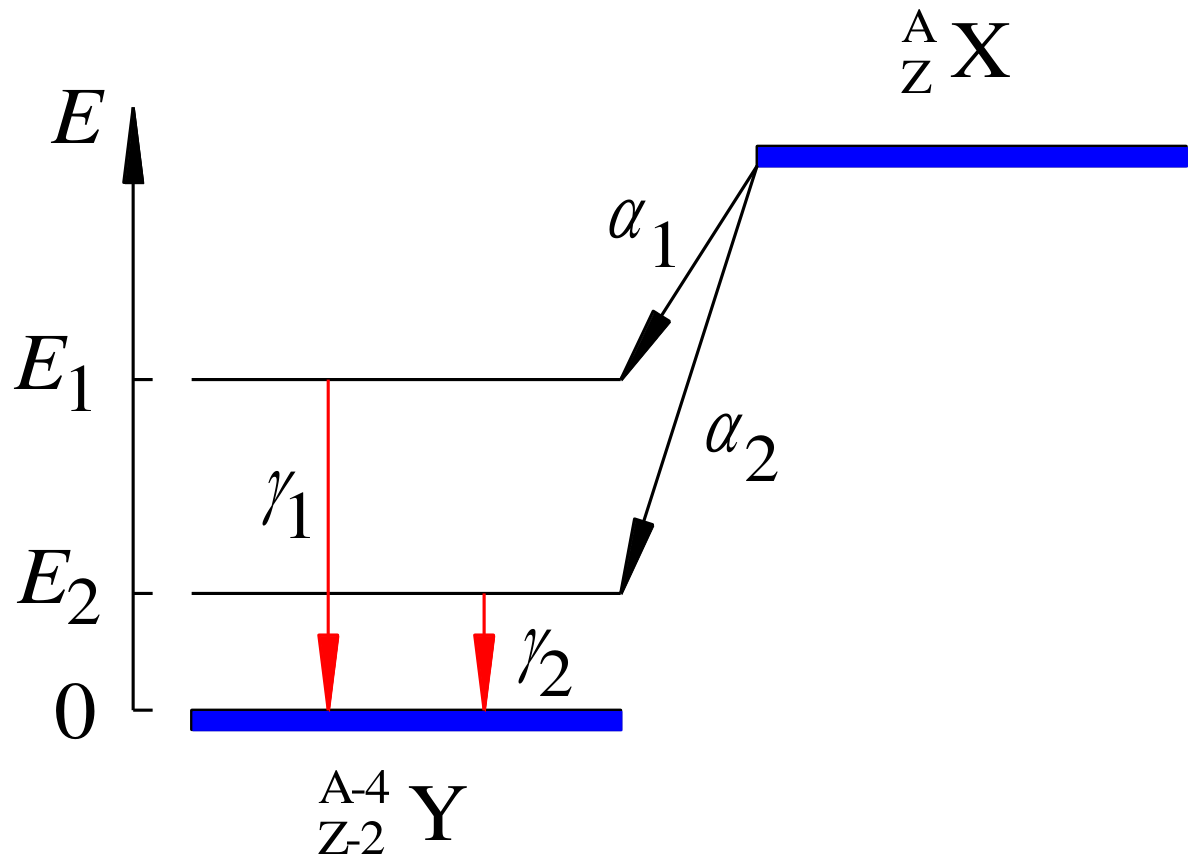
\includegraphics[width=0.3\linewidth]{theory/alpha-zerfall-schema}
    \caption{Schema eines $\alpha$-Zerfalls des Kerns X. In diesem Beispiel gibt
    es zwei $\alpha$-Zerfallskanäle, bei denen die $\alpha$-Teilchen $\alpha_1$
    oder $\alpha_2$ emittiert werden und bei denen zwei unterschiedliche 
    Energieniveaus $E_1$ und $E_2$ des Tochterkerns Y bevölkert werden. Der 
    Übergang von den Energieniveaus $E_1$ und $E_2$ in den Grundzustand von Y, 
    der per Definition die Energie 0 hat, erfolgt in diesem Beispiel unter 
    Emission der Gammaquanten $\gamma_1$ bzw. $\gamma_2$. Die energetischen 
    Grundzustände der Kerne sind blau gezeichnet\\ \textsc{Quelle:} \cite[S. 30, Abb. 1]{script}}
    \label{fig:Schema Alpha-Zerfall}
\end{figure}
\end{document}